\usepackage{../pvm}

\usetikzlibrary{shadows,shapes.multipart}

\title{Arrays}
\author{Fr\'ed\'eric Vogels}


\begin{document}

\begin{frame}
  \titlepage
\end{frame}

\begin{frame}
  \frametitle{C-style Arrays}
  \begin{itemize}
    \item Syntactically resemble Java arrays
    \item Arrays in Java are evil (too unflexible, use {\tt ArrayList})
    \item Arrays in \cpp\ are particularly evil
    \item Complicated rules
    \item ``Shortcuts'' that complicate things even more
  \end{itemize}
\end{frame}

\begin{frame}
  \frametitle{Quick Intermezzo: {\tt sizeof}}
  \begin{itemize}
    \item \cpp\ has {\tt sizeof({\it id})} operator
    \item Can be used to find out size
    \item Works on \emph{static} type
  \end{itemize}
  \code[font size=\small,frame=lines,width=.9\linewidth]{sizeof-examples.cpp}
\end{frame}

\begin{frame}
  \frametitle{Quiz: What's the Output?}
  \code[font size=\small,frame=lines,width=.9\linewidth]{sizeof-array.cpp}
\end{frame}

\begin{frame}
  \frametitle{Reasoning: Arrays as Pointers}
  \begin{itemize}
    \item When a {\tt T[]} is passed as parameter, its type decays to {\tt T*}
    \item The pointer points to the first element in the array
    \item You can also index pointers: {\tt p[0]} is same as {\tt *p}
    \item No way of knowing how large the array is
    \item Solution: pass along size as extra parameter
    \item Not knowing size is typical cause of buffer overflows
  \end{itemize}
\end{frame}

\begin{frame}
  \frametitle{Arrays as Pointers}
  \begin{center}
    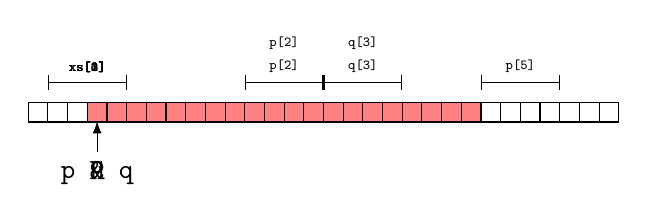
\begin{tikzpicture}[scale=.25]
      \only<2->{
        \draw[fill=red!50] (3,0) rectangle ++(20,1);
      }
      \visible<2>{
        \foreach \i in {0,...,4} {
          \tikzmath{
            int \x;
            \x = int(\i * 4 + 3);
          }

          \draw[|-|] (\x,2) -- ++(4,0) node[midway,above,font=\tiny] {\tt xs[\i]};
        }
      }

      \visible<3|handout:0>{
        \draw[-latex] (3.5,-1.5) -- ++(0,1.5) node[anchor=north,at start] {\tt p};
      }

      \visible<4|handout:0>{
        \draw[-latex] (3.5,-1.5) -- ++(0,1.5) node[anchor=north,at start] {\tt q};
      }

      \visible<5|handout:0>{
        \draw[|-|] (11,2) -- ++(4,0) node[midway,above,font=\tiny] {\tt p[2]};;
      }

      \visible<6|handout:0>{
        \draw[|-|] (15,2) -- ++(4,0) node[midway,above,font=\tiny] {\tt q[3]};;
      }

      \visible<7>{
        \draw[|-|] (23,2) -- ++(4,0) node[midway,above,font=\tiny] {\tt p[5]};;
      }
      
      \visible<0|handout:1>{
      	\draw[-latex] (3.5,-1.5) -- ++(0,1.5) node[anchor=north,at start] {\tt p \& q};
      	
      	\node[draw=none,fill=none,font=\tiny] at (13,4) {\tt p[2]};
      	
      	\node[draw=none,fill=none,font=\tiny] at (17,4) {\tt q[3]};
      }

      \draw (0,0) grid (30,1);
    \end{tikzpicture}
  \end{center}
  \vskip5mm
  \code[frame=lines,width=.5\linewidth]{arrays-as-pointers.cpp}
\end{frame}

\begin{frame}
  \frametitle{Old Version}
  \code[font size=\small,frame=lines,width=.9\linewidth]{sizeof-array2.cpp}
\end{frame}

\begin{frame}
  \frametitle{Improved Version}
  \code[font size=\small,frame=lines,width=.9\linewidth]{sizeof-array2-improved.cpp}
\end{frame}


\begin{frame}
  \frametitle{Quiz: What's the Problem?}
  \code[font size=\small,frame=lines,width=.9\linewidth]{return-array.cpp}
  \begin{tikzpicture}[overlay,remember picture]
    \only<2>{
      \draw[ultra thick,red] (rettype) circle (.5);
    }
  \end{tikzpicture}
\end{frame}

\begin{frame}
  \frametitle{Answer}
  \Large
  \begin{itemize}
    \item It doesn't compile
    \item Cannot return arrays
    \item Use pointer instead
   \end{itemize}
\end{frame}

\begin{frame}
  \frametitle{Quiz: What's the Problem?}
  \code[font size=\small,frame=lines,width=.9\linewidth]{return-array2.cpp}
\end{frame}

\begin{frame}
  \frametitle{Answer}
  \structure{Problem \#1}
  \begin{itemize}
    \item Array is created on stack
    \item Array size needs to be known at compile time
    \item Heap allocation is necessary
  \end{itemize}
  \vskip5mm
  \structure{Problem \#2}
  \begin{itemize}
    \item Array is created on stack
    \item Memory gets deallocated upon function exit
    \item You've got yourself a dangling pointer
  \end{itemize}
  \vskip5mm
  \structure{Problem \#3}
  \begin{itemize}
    \item Array size is unknown
    \item {\tt for} loop cannot possibly know when to stop iterating
  \end{itemize}
\end{frame}

\begin{frame}
  \frametitle{Array Heap Allocation}
  \structure{Allocation}
  \begin{center} \tt
    T* xs = new T[n];
  \end{center}
  \vskip5mm
  \structure{Allocation}
  \begin{center} \tt
    delete[] xs;
  \end{center}
  \begin{itemize}
    \item Don't forgot the {\tt []} when deallocating arrays!
  \end{itemize}
\end{frame}

\begin{frame}
  \frametitle{Improved Version}
  \code[font size=\small,frame=lines,width=.9\linewidth]{return-array2-improved.cpp}
\end{frame}

\begin{frame}
  \frametitle{\cpp\ Alternatives}
  \structure{Static Arrays (size known at compile time)}
  \begin{center} \tt
    std::array<T, N>
  \end{center}
  \vskip5mm
  \structure{Dynamic List}
  \begin{center} \tt
    std::vector<T>
  \end{center}
\end{frame}

\begin{frame}
  \frametitle{\tt std::array<T, N>}
  \begin{center}
    \begin{tabular}{ll}
      \bf Type & {\tt std::array<T, N>} \\[2mm]
      \bf Initialisation & {\tt std::array<T, N> \{ a,b,c,\dots \}} \\[2mm]
      \bf Reading & {\tt x = xs[i]} \\[2mm]
      \bf Writing & {\tt xs[i] = x} \\[2mm]
      \bf Size & {\tt xs.size()} \\
    \end{tabular}
  \end{center}
\end{frame}

\begin{frame}
  \frametitle{\tt std::array<T, N>}
  \code[frame=lines,font size=\small,width=.9\linewidth]{array-usage.cpp}
\end{frame}

\begin{frame}
  \frametitle{Quiz}
  \code[frame=lines,font size=\small,width=.9\linewidth]{by-value.cpp}
\end{frame}

\begin{frame}
  \frametitle{\tt std::array<T, N>}
  \begin{itemize}
    \item {\tt std::array}s are allocated on the stack
    \item {\tt std::array}s are passed by value
    \item For more efficiency: pass by pointer
  \end{itemize}
  \code[frame=lines,font size=\small,width=.9\linewidth]{by-pointer.cpp}
\end{frame}

\begin{frame}
  \frametitle{\tt std::array<T, N>}
  \begin{itemize}
    \item Functions can only deal with one array size
    \item Quite limiting
    \item Make functions polymorphic in size
  \end{itemize}
  \code[frame=lines,font size=\small,width=.9\linewidth]{polymorphic.cpp}
\end{frame}

\begin{frame}
  \frametitle{\tt std::vector<T>}
  \begin{center}
    \begin{tabular}{ll}
      \bf Type & {\tt std::vector<T>} \\[2mm]
      \bf Initialisation & {\tt std::vector<T> \{ a,b,c,\dots \}} \\[2mm]
      \bf Reading & {\tt x = xs[i]} \\[2mm]
      \bf Writing & {\tt xs[i] = x} \\[2mm]
      \bf Reading (with range check) & {\tt x = xs.at(i)} \\[2mm]
      \bf Writing (with range check) & {\tt xs.at(i) = x} \\[2mm]
      \bf Size & {\tt xs.size()} \\[2mm]
      \bf Add at end & {\tt xs.push\_back(x)} \\[2mm]
      \bf Remove at end & {\tt xs.pop\_back(x)} \\[2mm]
      \bf \vdots
    \end{tabular}
  \end{center}
\end{frame}

\begin{frame}
  \frametitle{\tt std::vector<T>}
  \code[frame=lines,font size=\small,width=.9\linewidth]{vector-usage.cpp}
\end{frame}

\begin{frame}
  \frametitle{\tt std::vector<T>}
  \begin{itemize}
    \item Same rules as with {\tt std::array}
    \item Pass-by-value
          \begin{itemize}
            \item Copied when passed as parameters \cake
            \item Copied when returned \cake
          \end{itemize}
    \item Use pointers for efficiency
  \end{itemize}
\end{frame}

\end{document}


%%% Local Variables:
%%% mode: latex
%%% TeX-master: "arrays"
%%% End:
